\documentclass[11pt,a4paper]{article}
\usepackage[margin=2.2cm]{geometry}
\usepackage[T1]{fontenc}
\usepackage{lmodern}
\usepackage{graphicx}
\usepackage{booktabs}
\usepackage{tabularx}
\usepackage{amsmath}
\usepackage{siunitx}
\usepackage{xcolor}
\usepackage{tikz}
\usetikzlibrary{positioning,fit,arrows.meta,backgrounds}
\usepackage{caption}
\usepackage{subcaption}
\usepackage[hidelinks]{hyperref}
\usepackage{enumitem}
\setlist{nosep,leftmargin=*}
\graphicspath{{../docs/figures/}}
\sisetup{group-separator={,}}
\captionsetup{font=small,labelfont=bf}
\emergencystretch=3em

\title{Air-Gapped Geospatial Inference for Multi-Sensor Imagery:\\
SAR + Optical Building Segmentation on SpaceNet~6\\[4pt]
\large DIP Course Project HSR-AIML-034}
\author{Aditya Singh}
\date{November 2026}

\begin{document}
\maketitle

\begin{abstract}
Defence and government users of satellite imagery often have to run analysis on networks
with no internet access. This project builds such a system end to end and measures it. The
image-processing core takes large SAR and optical GeoTIFF scenes, normalises and
despeckles them, cuts them into overlapping tiles, runs a U-Net building-segmentation
model in GPU batches, blends the tiles back into one seamless georeferenced probability map,
cleans it with mathematical morphology and turns it into building polygons. The core is
wrapped in an offline service (FastAPI, PostGIS, a GPU worker, Docker) that installs from a
single checksummed bundle without any network.
On SpaceNet~6 Rotterdam (0.5\,m SAR and optical), every DIP choice is measured
against a baseline. Hann-window overlap stitching removes tile seams (seam score
$3.23 \to 0.99$) and adds $+0.009$ IoU on the official validation extent. A per-acquisition
SAR normalisation is the best of five SAR pre-processing arms. Morphological clean-up raises
SAR object F1 from 0.223 to 0.244. SAR + optical fusion trained with synthetic clouds keeps
a pixel IoU of 0.527 at 80\,\% cloud cover, where a clean-trained optical model falls to 0.008.
FP16 inference gives the same accuracy as FP32 on two GPUs, a 4\,GB laptop card and a 96\,GB
data-centre card. Under replayed analyst traffic, batching tiles across jobs gives 30\,\%
more throughput and 2.3$\times$ lower median latency than per-job batching. A priority
queue with slow ageing cuts the 95th-percentile latency of urgent jobs by 89\,\% at
saturation.
\end{abstract}

\section{Introduction}
\label{sec:intro}

GalaxEye Space builds satellites that carry a SAR and a multispectral optical sensor on one
platform. SAR sees through cloud and at night but is hard to read (speckle, layover,
shadow); optical imagery is easy to read but useless under cloud. The problem statement
(HSR-AIML-034) asks for an inference platform for such multi-sensor imagery that runs
offline, with tiling, batching, GPU scheduling and an accuracy/speed analysis.

A scene is far larger than a GPU input (the optical mosaic used here is 369\,Mpx), so
every production system has to tile the scene, run the model per tile and stitch the
results. This is where most of the image processing lies. The project treats that
pipeline as the main subject and the service as the way it is delivered.

\paragraph{Contributions.}
\begin{enumerate}
\item A windowed raster pipeline (COG I/O, normalisation, Lee despeckling, overlap tiling
with reflect padding, weighted stitching with a disk-backed accumulator, morphology,
vectorisation) that never loads a full scene into memory. Every stage is unit-tested on
synthetic arrays and keeps the input georeferencing.
\item Four baseline-vs-improved studies with intermediate images:
S1 stitching, S2 normalisation and despeckling, S3 sensor fusion and cloud robustness,
S4 inference engines and the tile/overlap trade-off.
\item SAR, optical and fused U-Nets trained on a geographic split, with the SAR look direction
handled explicitly (Decision D5) and synthetic-cloud augmentation.
\item An air-gapped service: REST API, PostGIS job queue and result store, a GPU worker
with cross-job dynamic batching and priority scheduling with ageing, Docker images and an
offline bundle with a SHA-256 manifest. A clean install ran air-gapped jobs that returned
polygons (Gate~3).
\item Serving experiments: inference engines and batch size on two GPUs, and latency
against offered load, batching policy and priority policy on the laptop stack.
\end{enumerate}

\section{Existing work and what is different here}
\label{sec:related}

\paragraph{SpaceNet~6 / MSAW.}
The SpaceNet~6 challenge \cite{shermeyer2020sn6} released half-metre quad-polarisation
airborne SAR and WorldView-2 optical imagery over Rotterdam with about 48\,000 building
footprints. The winning solutions segmented buildings from SAR with ensembles of U-Net
style networks, used optical imagery only for pre-training, and rotated or flipped the SAR
by look direction. They were scored on per-tile building F1 and ran offline on fixed test
tiles.

\paragraph{Tiling and stitching.}
Overlap-tile inference goes back to the original U-Net \cite{ronneberger2015unet}, which
predicts only the valid centre of each tile. Weighted blending of overlapping predictions
(for example with a raised-cosine window) is a widespread practice in remote-sensing
segmentation tools, but it is usually applied without measuring what it buys.

\paragraph{Cloud-hosted geospatial ML.}
Commercial platforms run large-raster inference in the cloud with managed storage and
autoscaling. They assume network access, which is exactly what an air-gapped site lacks.

\paragraph{What this project adds.}
\begin{itemize}
\item \textbf{Scene-level DIP evidence, not only tile scores.} Stitching is measured on whole
mosaics (40\,Mpx and 121\,Mpx) with a seam score and a border-band IoU, so the effect of each
stitching strategy is visible and quantified (S1).
\item \textbf{SAR pre-processing as a controlled study.} Linear vs dB, Lee 5$\times$5 vs
7$\times$7, global vs per-acquisition statistics, over three seeds (S2). The challenge
entries did not report this comparison.
\item \textbf{Fusion judged by robustness, not only accuracy.} Fusion barely changes clear-sky
IoU, but with cloud augmentation it keeps working where optical fails (S3).
\item \textbf{Deployment as a measured system.} The same pipeline runs inside an offline
service with a queue, a scheduler and a bundle installer. Throughput and latency are
measured under replayed traffic, and FP16/TensorRT are measured on an edge-class and a
data-centre GPU (S4, E1--E4).
\end{itemize}

\section{Data}
\label{sec:data}

\paragraph{Source.} SpaceNet~6 AOI 11 Rotterdam, CC BY-SA 4.0
\cite{shermeyer2020sn6}. Each 450\,m tile has a 4-band SAR-Intensity image (HH, HV, VH, VV, in
dB) and a pan-sharpened 4-band optical image (R, G, B, NIR, 16-bit), both at 0.5\,m on the
same grid, plus building footprints. The train archive (D2, 3401 tiles, 39\,GiB) and the
pan-sharpened TrainVal optical mosaic (D3, 369\,Mpx) were used. Raw data stays read-only on
an external drive and is versioned with DVC.

\paragraph{Geographic split (Decision D1).} The D2 tiles cover only the western 85\,\% of the
official Train extent, so splits are cut west to east inside that coverage: train 1798, tune
349 (model selection and threshold) and val 637 tiles. Tiles crossing a split boundary are
dropped (617), so no tile appears in two splits (Fig.~\ref{fig:splits}).

\paragraph{Large scenes.}
\textbf{D4} (Decision D3) is a mosaic of all 637 val tiles, 2621$\times$15451\,px (40\,Mpx), with
labels and a per-pixel record of the source strip, built with whole-pixel pasting so SAR
and optical stay co-registered. \textbf{D3-val} is the D3 optical mosaic cut to the
official validation extent (121\,Mpx) with the All-Val labels.

\paragraph{Look direction.} Each SAR strip looks north or south, so building layover points
opposite ways in the two groups. The measured SAR-to-optical offset depends on the look
direction (Decision D2), and the SAR and fused models therefore see every strip in the same
orientation (D5).

\begin{figure}[t]
\centering
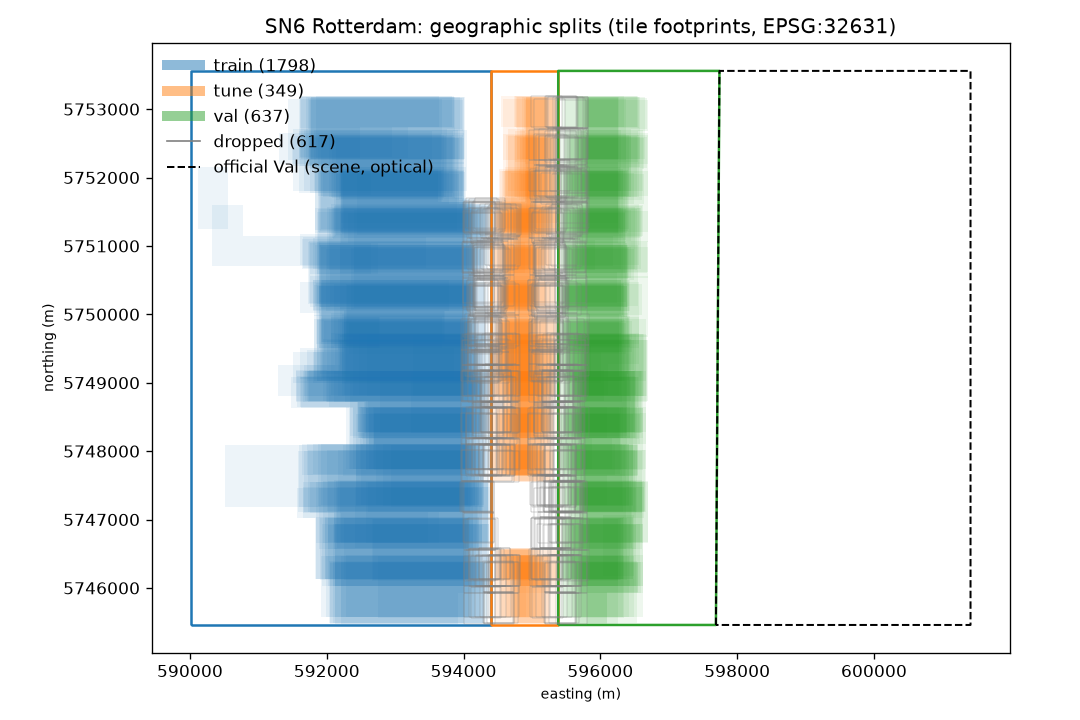
\includegraphics[width=0.48\linewidth]{splits_map.png}\hfill
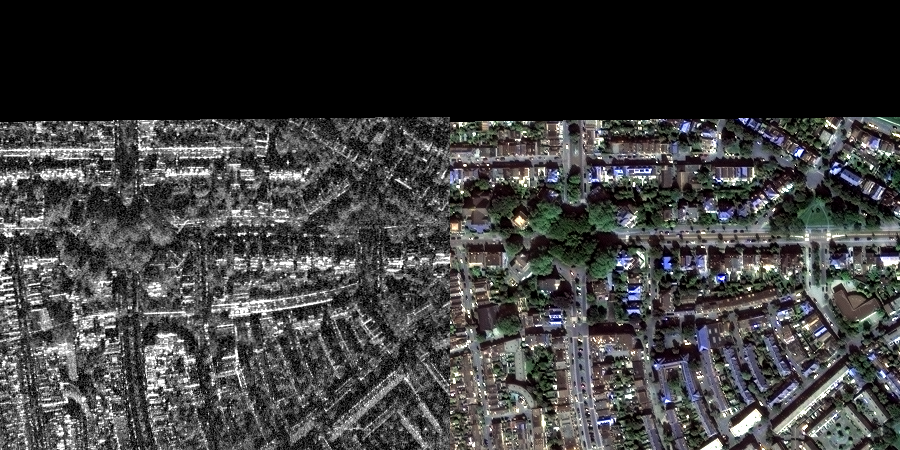
\includegraphics[width=0.48\linewidth]{gate0_sar_optical.png}
\caption{Left: geographic train / tune / val split inside the covered extent. Right: one
SAR tile (dB) and its optical twin.}
\label{fig:splits}
\end{figure}

\section{System overview}
\label{sec:system}

Figure~\ref{fig:block} shows where the DIP and AI/CV stages sit. The shaded block is the
graded image-processing core (\texttt{src/geoinfer/\{io, preprocess, tiling, postprocess,
eval\}}). Everything else is the delivery vehicle.

\begin{figure}[t]
\centering
\resizebox{\linewidth}{!}{%
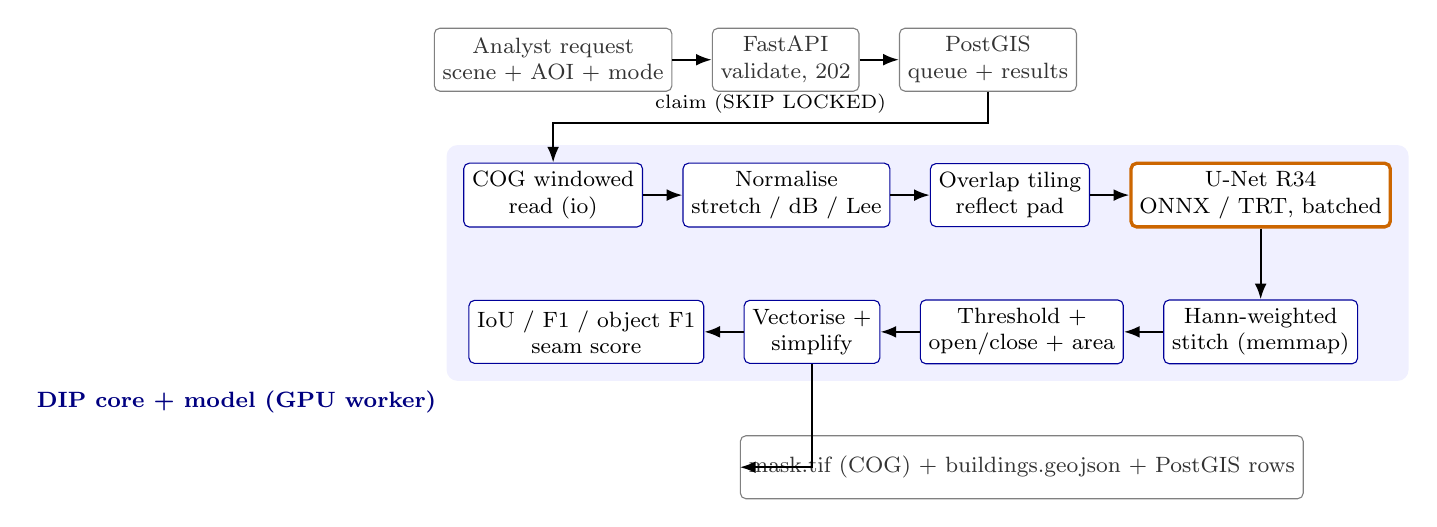
\begin{tikzpicture}[
  node distance=4mm and 5mm,
  box/.style={draw, rounded corners=2pt, align=center, font=\footnotesize,
              minimum height=8mm, inner sep=3pt, fill=white},
  dip/.style={box, draw=blue!60!black},
  ai/.style={box, draw=orange!80!black, very thick},
  svc/.style={box, draw=black!50, text=black!80},
  arr/.style={-{Latex[length=2mm]}, thick}]
\node[svc] (req) {Analyst request\\scene + AOI + mode};
\node[svc, right=of req] (api) {FastAPI\\validate, 202};
\node[svc, right=of api] (db) {PostGIS\\queue + results};
\node[dip, below=9mm of req] (io) {COG windowed\\read (io)};
\node[dip, right=of io] (norm) {Normalise\\stretch / dB / Lee};
\node[dip, right=of norm] (tile) {Overlap tiling\\reflect pad};
\node[ai, right=of tile] (unet) {U-Net R34\\ONNX / TRT, batched};
\node[dip, below=9mm of unet] (stitch) {Hann-weighted\\stitch (memmap)};
\node[dip, left=of stitch] (morph) {Threshold +\\open/close + area};
\node[dip, left=of morph] (vec) {Vectorise +\\simplify};
\node[dip, left=of vec] (eval) {IoU / F1 / object F1\\seam score};
\node[svc, below=9mm of morph] (out) {mask.tif (COG) + buildings.geojson + PostGIS rows};
\begin{scope}[on background layer]
\node[fill=blue!6, rounded corners=4pt, inner sep=6pt,
      fit=(io)(norm)(tile)(unet)(stitch)(morph)(vec)(eval),
      label={[font=\footnotesize\bfseries, text=blue!50!black]south west:DIP core + model (GPU worker)}] {};
\end{scope}
\draw[arr] (req) -- (api);
\draw[arr] (api) -- (db);
\draw[arr] (db.south) |- ++(0,-4mm) -| node[pos=0.25, above, font=\scriptsize]{claim (SKIP LOCKED)} (io.north);
\draw[arr] (io) -- (norm);
\draw[arr] (norm) -- (tile);
\draw[arr] (tile) -- (unet);
\draw[arr] (unet) -- (stitch);
\draw[arr] (stitch) -- (morph);
\draw[arr] (morph) -- (vec);
\draw[arr] (vec) -- (eval);
\draw[arr] (vec.south) |- (out.west);
\end{tikzpicture}}
\caption{Block diagram. Blue: DIP operations; orange: the learnt model; grey: service
components. The worker claims a job from the PostGIS queue and runs the shaded pipeline;
evaluation runs on held-out data only.}
\label{fig:block}
\end{figure}

\section{Image-processing pipeline}
\label{sec:dip}

\subsection{Raster I/O}
All reads are windowed (\texttt{rasterio} windows, a hard limit on window size), so no stage
reads a whole scene. Outputs are tiled, compressed Cloud-Optimised GeoTIFFs written to a
temporary name and renamed on success, and every output keeps the input CRS and
transform (checked in the tests).

\subsection{Normalisation and despeckling (study S2)}
\paragraph{Optical.} Two arms: per-tile min-max, and a global 2--98\,\% percentile stretch
plus z-score with train-split statistics.
\paragraph{SAR.} SAR intensity has multiplicative speckle and a heavy-tailed distribution,
so five arms are compared:
\begin{itemize}
\item linear intensity;
\item dB;
\item Lee filter \cite{lee1980} 5$\times$5 or 7$\times$7, on linear intensity and then
converted to dB, with the equivalent number of looks (ENL) estimated from homogeneous
train windows;
\item per-acquisition (per-strip) clip and z-score statistics (Decision D4).
\end{itemize}
The D4 mosaic showed median SAR levels spanning 29\,dB across strips, which a single global
normalisation cannot remove (Fig.~\ref{fig:s2}).

\begin{figure}[t]
\centering
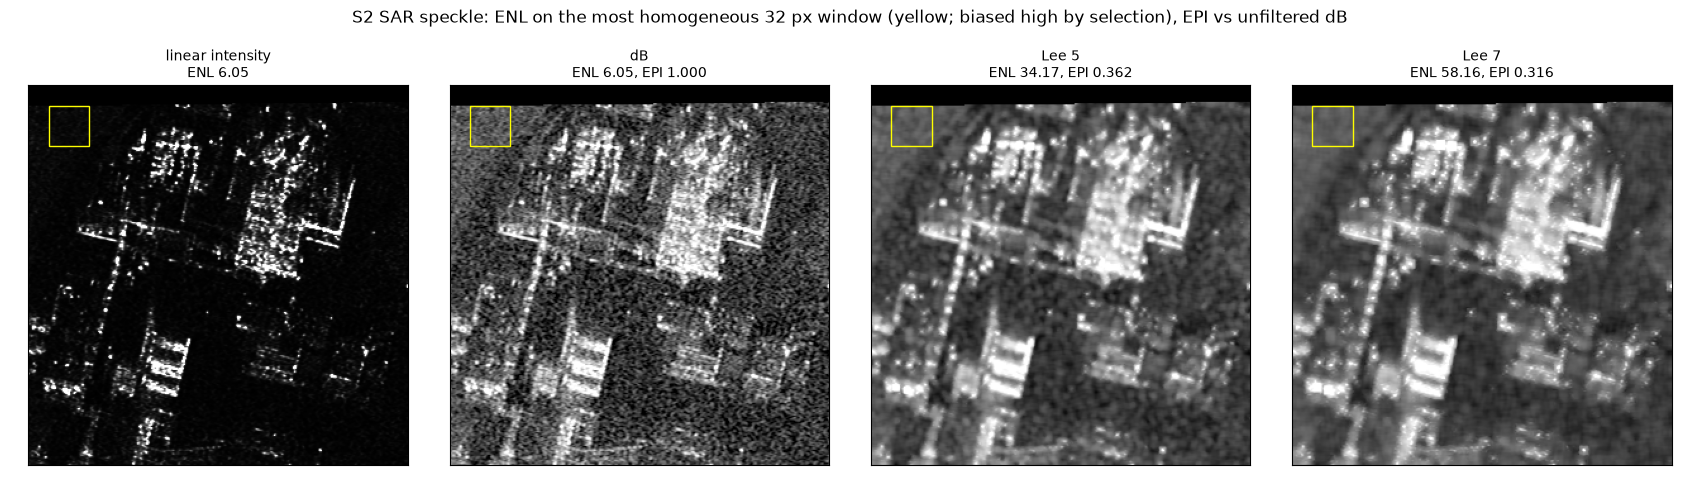
\includegraphics[width=0.49\linewidth]{s2_sar_patch.png}\hfill
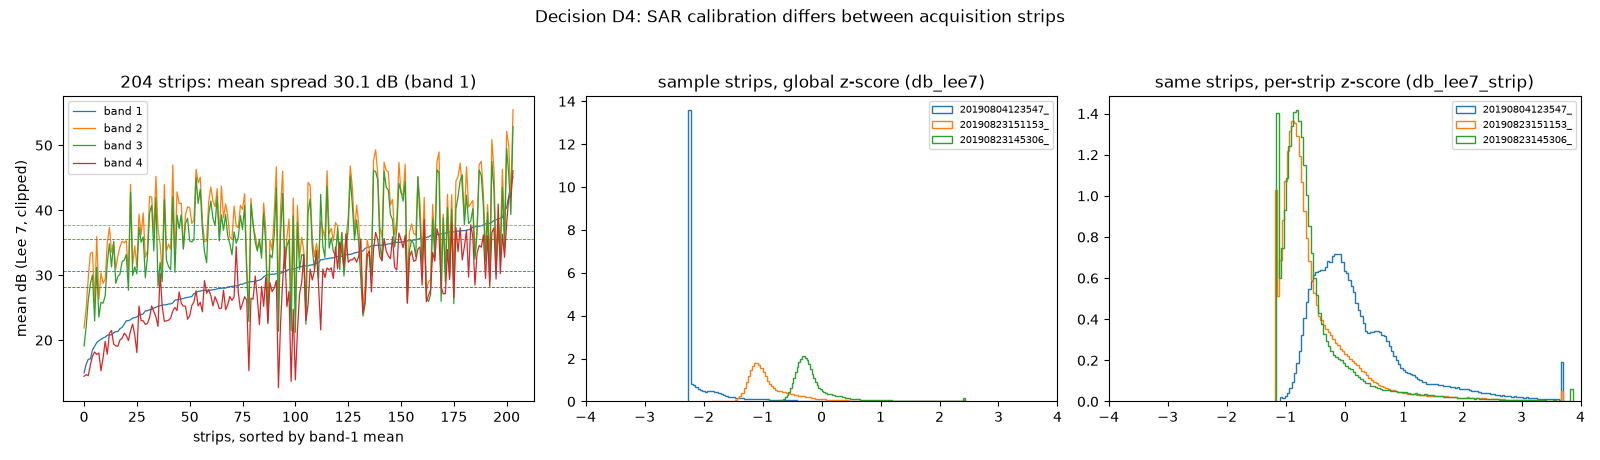
\includegraphics[width=0.49\linewidth]{s2_strip_calibration.png}
\caption{S2 intermediate images. Left: one SAR patch as linear intensity, dB, and dB after
Lee 5$\times$5 and 7$\times$7: speckle drops while building edges stay. Right: per-strip SAR
levels in D4 and the effect of per-strip normalisation.}
\label{fig:s2}
\end{figure}

\subsection{Tiling and stitching (study S1)}
The grid starts half an overlap outside the scene and steps by $T-O$, so the tile centres
partition the scene exactly. Tiles crossing the scene edge are filled by mirror reflection
and the padded pixels are marked invalid. Four strategies combine tile predictions:
\begin{itemize}
\item naive, $O=0$;
\item centre crop;
\item a Hann (raised-cosine) weighted average, with weights
$w(x,y) = \sin^2(\pi x/T)\sin^2(\pi y/T)$ restricted to the overlap ramps;
\item a Tukey weighted average.
\end{itemize}
Scenes above 50\,Mpx accumulate the weighted sums in a memory-mapped file on disk.
Quality is measured with a seam score: the mean gradient of the probability map on tile
borders divided by the same off the borders, where 1.0 means no visible seam. A border-band
IoU, computed only within 32\,px of a tile edge, isolates the stitching effect.

\begin{figure}[t]
\centering
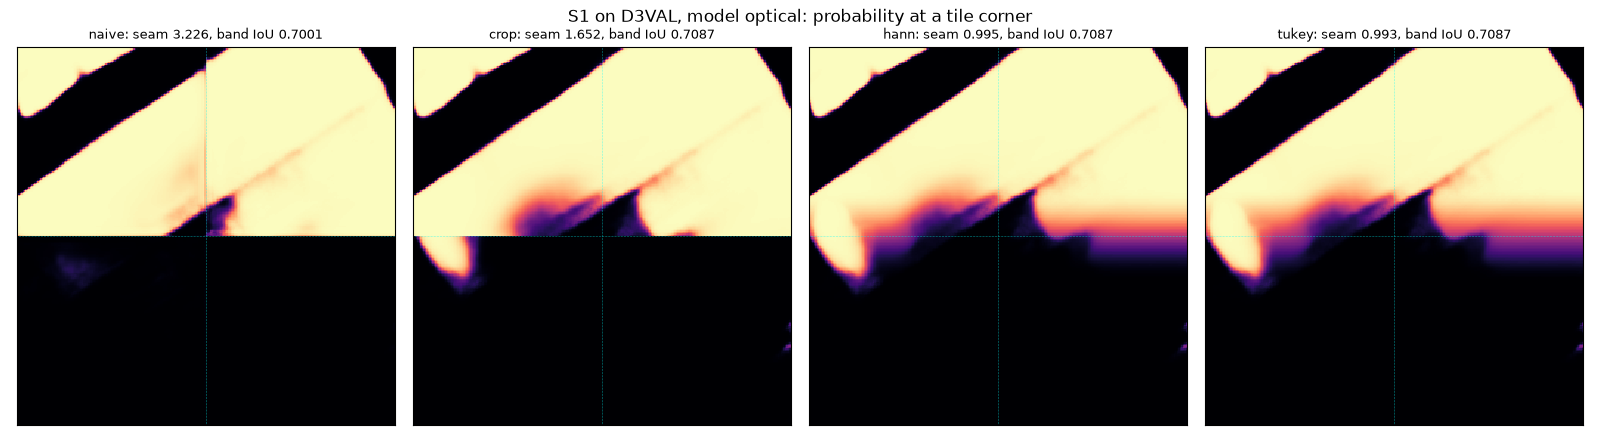
\includegraphics[width=\linewidth]{s1_d3val_optical.png}
\caption{S1 on the official validation extent (D3-val, 121\,Mpx), trained optical model. The
probability map at a tile corner: naive stitching shows a hard seam, while centre crop, Hann
and Tukey blending remove it.}
\label{fig:s1}
\end{figure}

\subsection{Post-processing and vectorisation}
Probabilities are thresholded at the threshold tuned on the tune split. A 3$\times$3 opening
removes specks, a 3$\times$3 closing fills roof holes, and components under 20\,m$^2$ are
removed (4-connectivity, so diagonally touching buildings stay apart). The clean-up runs in
blocks with a halo, so it scales to whole scenes. The mask is then traced into polygons
block-wise, merged across block borders and simplified with Douglas--Peucker (0.5\,m).
Polygons are exported as GeoJSON in EPSG:4326 and inserted into PostGIS
(Fig.~\ref{fig:post}).

\begin{figure}[t]
\centering
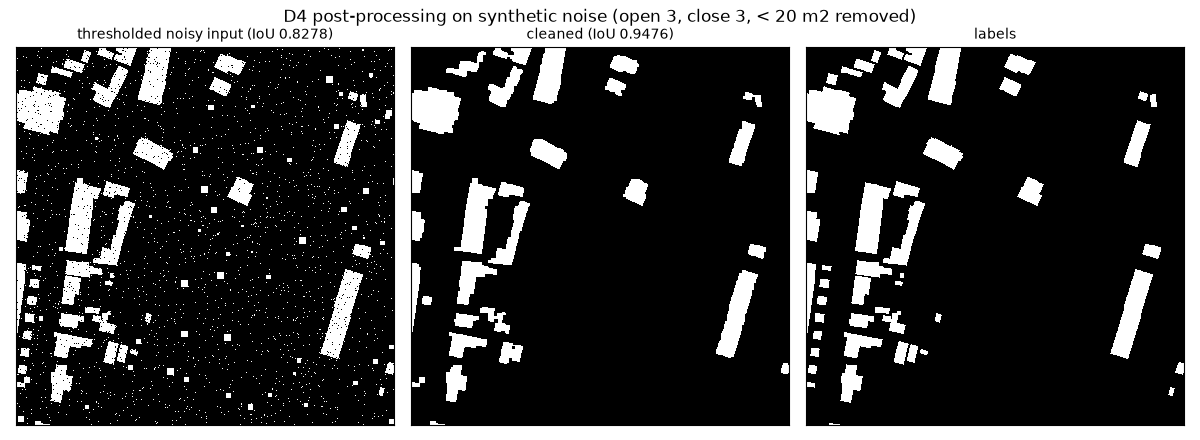
\includegraphics[width=0.8\linewidth]{postprocess_d4.png}
\caption{Morphological clean-up on D4 with synthetic noise: thresholded mask, after
opening/closing, after small-component removal, and the traced polygons.}
\label{fig:post}
\end{figure}

\subsection{Metrics}
Pixel IoU, F1, precision and recall are reported on the building class. Object F1 follows
the SpaceNet convention: a predicted polygon matches a ground-truth polygon at polygon
IoU $\ge 0.5$, and buildings under 20\,m$^2$ are ignored. Seam score and border-band IoU
measure stitching.

\section{Models}
\label{sec:models}
All three models are U-Nets \cite{ronneberger2015unet} with a ResNet-34 encoder
\cite{he2016resnet} and ImageNet initialisation (Decision D6; the stem of a $C$-channel
input copies RGB weights, channel $i \leftarrow$ RGB weight $(i \bmod 3) \cdot 3/C$). The
inputs are optical (4 channels), SAR (4) and fused (8, optical first).

Training ran on the college server's RTX PRO 6000 (one GPU of two, shared):
\begin{itemize}
\item 30 epochs, batch 16, 512\,px random crops, AdamW (learning rate $3\cdot10^{-4}$);
\item BCE + Dice loss on valid pixels only, with mixed precision;
\item east-west flips only, so the SAR look direction is preserved;
\item look-direction-1 strips flipped north-south for SAR and fused (D5).
\end{itemize}
The cloud-trained variants add synthetic clouds (fractal noise, soft edges, cover up to
80\,\%) to half of the optical training samples. The model is selected on tune IoU, and the
binarisation threshold is swept on tune. Models are exported to ONNX (opset 18, dynamic
batch and size) with a parity check against PyTorch: the largest logit difference is
$\le 2.7\cdot10^{-5}$.

\section{Experiments and results}
\label{sec:results}
All numbers are on the held-out val split or on the D4 / D3-val scenes built from held-out
data. Thresholds are tuned on the tune split. Full logs are in \texttt{docs/experiments.md}.

\subsection{S1: stitching}
\begin{table}[h]
\centering\small
\begin{tabular}{lrrrrr}
\toprule
& \multicolumn{2}{c}{D4 (40\,Mpx)} & \multicolumn{3}{c}{D3-val (121\,Mpx)}\\
\cmidrule(lr){2-3}\cmidrule(lr){4-6}
Strategy & Seam score & Border IoU & Seam score & Border IoU & Object F1\\
\midrule
Naive ($O=0$) & 2.79 & 0.704 & 3.23 & 0.700 & 0.539\\
Centre crop & 1.48 & 0.709 & 1.65 & 0.709 & 0.548\\
Hann (proposed) & \textbf{0.99} & \textbf{0.709} & \textbf{0.995} & \textbf{0.709} & \textbf{0.549}\\
Tukey & 0.98 & 0.709 & 0.993 & 0.709 & 0.549\\
\bottomrule
\end{tabular}
\caption{S1. Overlap stitching ($T=512$, $O=64$) removes the seams that naive tiling
leaves (seam score $\approx 1$). It also raises IoU near tile borders and object F1 on the
official validation extent. Crop removes only half of the seam; Hann and Tukey are
equivalent.}
\end{table}

\subsection{S2: normalisation and SAR despeckling}
\begin{table}[h]
\centering\small
\begin{tabular}{lrrr}
\toprule
SAR arm (3 seeds) & Val pixel IoU & Pixel F1 & Object F1\\
\midrule
Linear intensity (1 seed) & 0.403 & 0.575 & 0.148\\
dB (baseline) & 0.478 $\pm$ 0.009 & 0.647 & 0.256 $\pm$ 0.002\\
dB + Lee 5$\times$5 & 0.469 $\pm$ 0.007 & 0.639 & 0.232 $\pm$ 0.004\\
dB + Lee 7$\times$7 & 0.474 $\pm$ 0.004 & 0.643 & 0.248 $\pm$ 0.007\\
dB + Lee 7$\times$7, per strip (proposed) & \textbf{0.482 $\pm$ 0.009} & \textbf{0.650} &
\textbf{0.264 $\pm$ 0.005}\\
\bottomrule
\end{tabular}
\caption{S2, SAR. The dB transform is the largest step (+0.075 IoU over linear). Lee
filtering alone does not help a CNN that can learn its own smoothing. Per-acquisition
statistics are best on every metric. Optical: per-tile min-max and global stretch tie on
tile IoU (0.681 vs 0.682), but min-max leaves visible seams after stitching (seam score
2.60 vs 0.92), so the service uses the global stretch.}
\end{table}

\subsection{S3: sensor fusion and cloud robustness}
On clear imagery fusion adds little: val pixel IoU is optical 0.682, SAR 0.479 and fused
0.688, and object F1 is 0.508, 0.244 and 0.519. The value of SAR appears under cloud
(Table~\ref{tab:s3}, Fig.~\ref{fig:s3}). Models trained on clean optical collapse as clouds
cover the scene. Training with synthetic clouds keeps the optical model usable, and the
fused model degrades least: at 80\,\% cover it keeps 0.527 IoU, ahead of both optical
(0.502) and SAR alone (0.479).

\begin{table}[h]
\centering\small
\begin{tabular}{lrrrrr}
\toprule
Val pixel IoU at cloud cover & 0\,\% & 20\,\% & 40\,\% & 60\,\% & 80\,\%\\
\midrule
Optical, clean-trained (baseline) & 0.682 & 0.308 & 0.130 & 0.042 & 0.008\\
Fused, clean-trained & 0.688 & 0.382 & 0.189 & 0.078 & 0.025\\
SAR only & 0.479 & 0.479 & 0.479 & 0.479 & 0.479\\
Optical, cloud-trained & 0.686 & 0.654 & 0.623 & 0.578 & 0.502\\
Fused, cloud-trained (proposed) & 0.680 & 0.644 & 0.614 & 0.577 & \textbf{0.527}\\
\bottomrule
\end{tabular}
\caption{S3. Cloud robustness; identical synthetic clouds for every model.}
\label{tab:s3}
\end{table}

\begin{figure}[t]
\centering
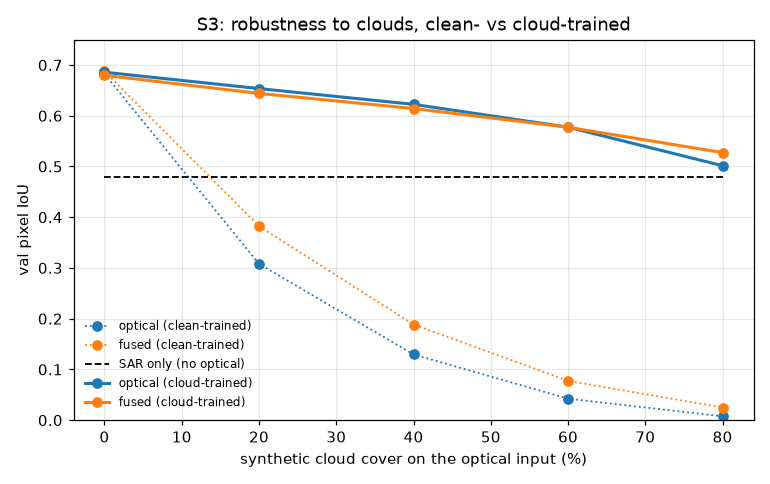
\includegraphics[width=0.75\linewidth]{s3_clouds_all.png}
\caption{S3: val pixel IoU against synthetic cloud cover.}
\label{fig:s3}
\end{figure}

\paragraph{Morphology.} Clean-up raises SAR object F1 from 0.223 to 0.244 (the closing joins
building fragments) and is neutral for optical and fused (within $\pm 0.005$). It costs up to
0.013 pixel IoU because it trims building edges.

\subsection{S4, E1, E5: inference engines, batch size, tile and overlap}
Five engines were run on identical, worker-normalised D4 tiles on two GPUs, with 50
warm-up batches and 3 timed repeats per configuration (Table~\ref{tab:s4},
Fig.~\ref{fig:s4}).

\begin{table}[h]
\centering\small
\resizebox{\linewidth}{!}{%
\begin{tabular}{llrrrrr}
\toprule
GPU & Engine & Best batch & Tiles/s & p95 batch (ms) & Pixel IoU & Object F1\\
\midrule
GTX 1650 (4\,GB) & PyTorch FP32 (baseline) & 4 & 36 & 113 & 0.710 & 0.503\\
 & PyTorch AMP / ORT FP16 & \multicolumn{5}{l}{non-finite output (FP16 overflow on this GPU)}\\
 & ORT CUDA FP32 & 1 & 27 & 43 & 0.710 & 0.503\\
 & TensorRT FP16 & 8 & \textbf{53} & 153 & 0.710 & 0.504\\
\midrule
RTX PRO 6000 (96\,GB) & PyTorch FP32 & 16 & 512 & 33 & 0.710 & 0.503\\
 & PyTorch AMP & 32 & \textbf{625} & 60 & 0.710 & 0.503\\
 & ORT CUDA FP32 & 1 & 317 & 3 & 0.710 & 0.503\\
 & ORT CUDA FP16 & 4 & 615 & 8 & 0.710 & 0.504\\
 & TensorRT FP16 & 4 & 522 & 9 & 0.710 & 0.504\\
\bottomrule
\end{tabular}}
\caption{S4 on 512\,px tiles. Accuracy is from whole-D4 runs through the service pipeline.
FP16 loses no accuracy. On the 4\,GB laptop GPU the network is the bottleneck (92--97\,\% GPU
utilisation, thermally throttled to 990\,MHz) and TensorRT FP16 doubles throughput. On the
server GPU utilisation stays at 23--55\,\%: host-side copies and the sigmoid limit
throughput, so the FP16 engines end up level.}
\label{tab:s4}
\end{table}

\begin{figure}[t]
\centering
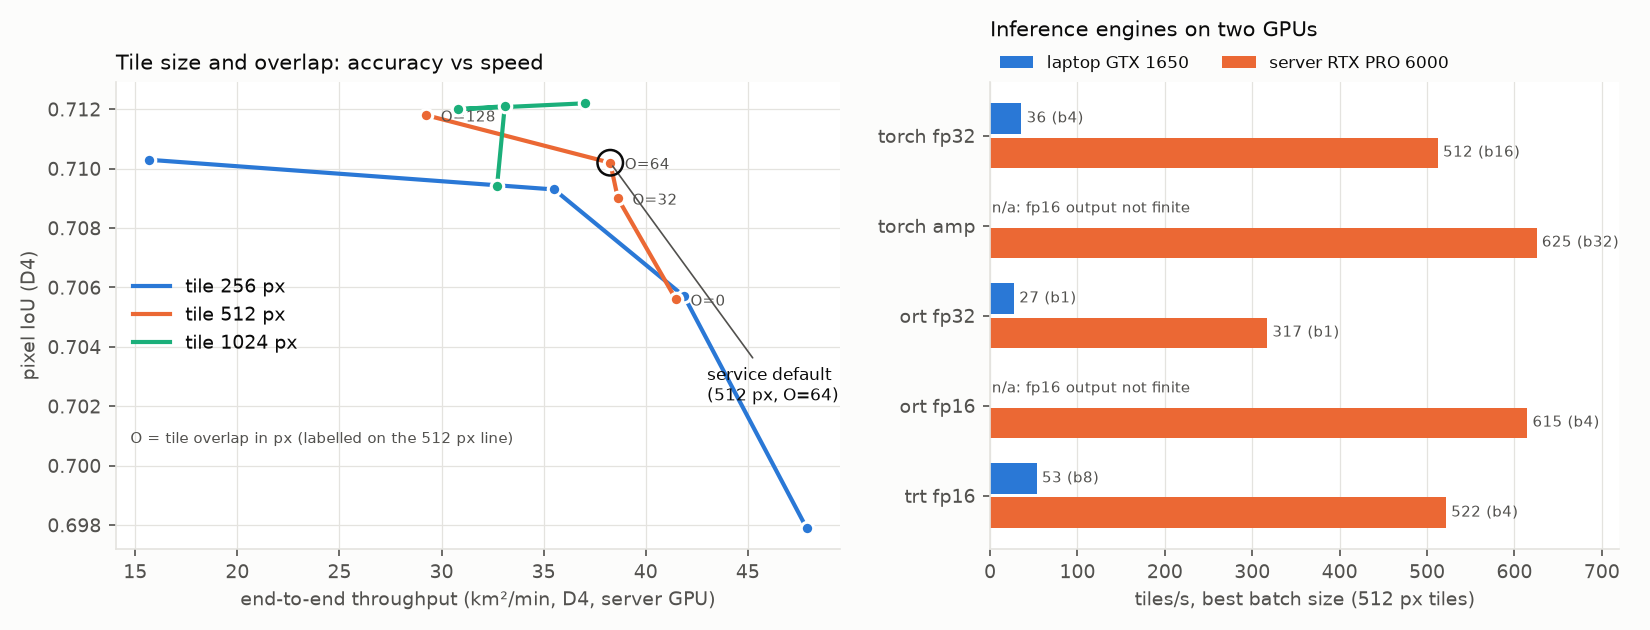
\includegraphics[width=\linewidth]{s4_pareto.png}
\caption{Left: tile size and overlap against end-to-end throughput on D4 (server GPU,
including reading, stitching and post-processing). Overlap always gains IoU; 256\,px tiles
without overlap lose 0.012. The service default (512\,px, $O=64$) sits within 0.002 of the
best IoU. Right: best engine throughput on the two GPUs.}
\label{fig:s4}
\end{figure}

\paragraph{End to end.} Inference is a small part of a whole-scene job. On D4 (10\,km$^2$)
the server processes 31--40\,km$^2$/min with any engine; on the laptop, model time is
6--12\,s of a 55--100\,s run, and reading tiles from the external drive and the CPU
post-processing dominate. Faster engines therefore pay off mainly in a server that keeps
the GPU busy across many jobs, which is the purpose of the scheduler below.

\subsection{E2--E4: serving under load}
\label{sec:serving}
% LOAD-RESULTS: filled from docs/figures/e_load_laptop.json (scripts/plot_load.py)
\paragraph{Method.} The serving experiments replay one fixed sequence of 200 synthetic analyst
requests (\texttt{data/requests/requests\_seed42.jsonl}, seed 42):
\begin{itemize}
\item Poisson arrivals at unit rate, scaled to the target rate, so every run sees the same jobs;
\item 60\,\% optical jobs on the D3 mosaic with square AOIs of 0.5, 1 or 2\,km;
\item 40\,\% SAR or fused jobs on the demo band with 0.5 or 1\,km AOIs;
\item 20\,\% high priority (priority 5 against 0).
\end{itemize}
The replay is open-loop: each request is sent at its scheduled time, whatever the state of
earlier ones. A closed-loop generator such as Locust waits for each user's previous
request, which hides queueing delay at high load. Latency is taken from the database
timestamps, from submission to result ready.

Between runs, the worker is recreated with the arm's scheduling and the job tables are
emptied. Load is given in multiples of a capacity measured with a burst of 24 simultaneous
requests: 0.091\,jobs/s (Decision D8). The stack runs on the laptop: GTX 1650, WSL limited
to 4.8\,GB of RAM, worker container limited to 4\,GB. AOIs of 5\,km are left out for memory.

\paragraph{E4: latency against offered load.}
Latency stays flat up to 3$\times$ the burst capacity (0.27 jobs/s): p50 is 4--6\,s and
p95 is 8--14\,s, while throughput grows from 2 to 23\,km$^2$/min. At 4$\times$ the queue
builds (p50 95\,s, p95 266\,s) while throughput levels off at 22\,km$^2$/min, so the
saturation point lies between 0.27 and 0.37 jobs/s (Fig.~\ref{fig:load},
Table~\ref{tab:load}). The burst understates the sustainable rate: 24 jobs arriving at
once keep two jobs in flight all the time and fill the 4\,GB of GPU memory (peak
4056\,MiB), whereas steady arrivals rarely overlap below the knee. The GPU stays at
4--35\,\% utilisation throughout, because reading and normalising tiles (CPU) take most of
each job's time.

\paragraph{E2: batching policy at 3$\times$.}
Batching tiles across jobs is what keeps the service out of saturation. Per-job batches
(the baseline) reach 14.6\,km$^2$/min with p50 202\,s. Cross-job batches with a 10 or
25\,ms hold-back reach 18.4--19.2\,km$^2$/min (+30\,\%) with p50 84--89\,s
(2.3$\times$ lower). A 50\,ms hold-back is as bad as per-job batching (14.3\,km$^2$/min,
p50 199\,s): the GPU waits for batches to fill while jobs queue, and its utilisation drops
to 40\,\%.

\paragraph{E3: queue policy.}
The queue ranks jobs by $\text{priority} + a\cdot t_{\text{wait}}$.
\begin{itemize}
\item \textbf{At 4$\times$,} priority with ageing $a = 0.1$/s cuts the p95 latency of
high-priority jobs from 673\,s (FIFO) to 323\,s ($-52$\,\%) and their p50 from 484\,s to
184\,s. Normal jobs are no worse off: their p95 is 550\,s, against 704\,s under FIFO.
\item \textbf{At 3$\times$} that policy gives no gain (high-priority p95 125\,s for
both). With $a = 0.1$/s, a waiting normal job outranks a newly arrived high-priority job
after $5/0.1 = 50$\,s, and queue waits at this load exceed that, so the order is close to
FIFO. Ageing trades the responsiveness of high-priority work against a starvation bound.
\item \textbf{Slower ageing} ($a = 0.01$/s, so priority holds for 500\,s) gives the
clearest result. The p95 latency of high-priority jobs falls to 40\,s at 3$\times$
($-68$\,\% against FIFO) and to 74\,s at 4$\times$ ($-89$\,\%), with p50 of 16 and
33\,s. Normal jobs pay for it, but within the same order as FIFO: p95 158\,s against
109\,s at 3$\times$, and 551\,s against 704\,s at 4$\times$. Throughput stays close to
FIFO (17.6 against 18.3\,km$^2$/min at 3$\times$, 12.6 against 10.7 at 4$\times$),
because the policy only reorders the same work.
\end{itemize}

\paragraph{Caveats.} The laptop warmed from 72 to 89\,$^\circ$C over the session, and
per-job CPU time doubled with it. Comparisons are therefore made within an experiment,
whose arms ran back to back, and not across experiments. For example, the 3$\times$ point
of E4 ran cooler than the E2 arms at the same load. The Docker VM clock occasionally jumped
by 5\,h\,30\,min (UTC against IST). Those timestamps are corrected by the jump and
counted. After correction, every run's makespan agrees with its client-side wall time to
within 4\,\%.

\begin{figure}[t]
\centering
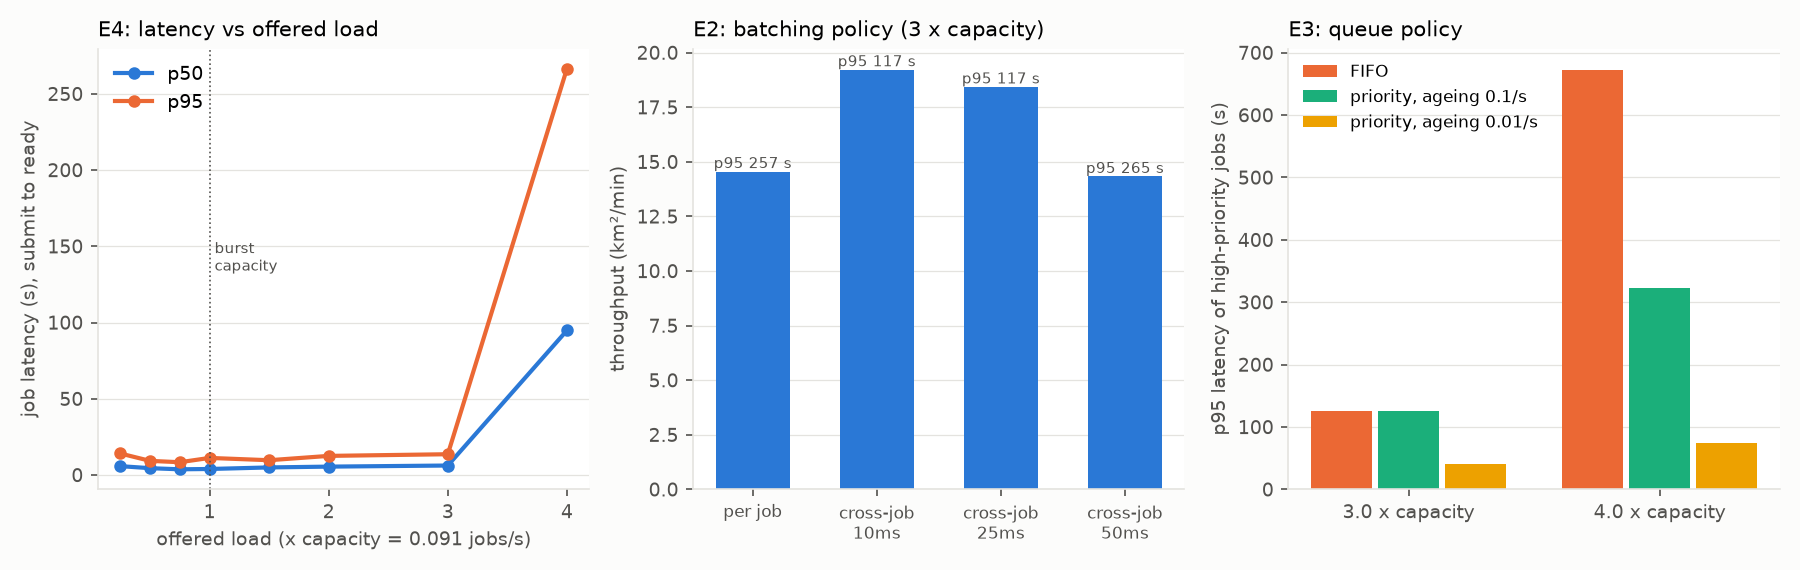
\includegraphics[width=\linewidth]{e_load.png}
\caption{Serving experiments on the laptop stack. Left: E4 job latency (p50, p95) against
offered load. Middle: E2 throughput by batching policy at 3$\times$ (labels: p95).
Right: E3 p95 latency of high-priority jobs by queue policy.}
\label{fig:load}
\end{figure}

\begin{table}[t]
\centering\small
\begin{tabular}{llrrrrrr}
\toprule
Exp. & Arm & Load & p50 (s) & p95 (s) & High-prio p95 (s) & km$^2$/min & GPU \\
\midrule
cap. & burst of 24 & burst & 125.6 & 235.4 & 39.6 & 8.6 & 63\,\% \\
E4 & cross-job 25 ms, priority & 0.25$\times$ & 5.8 & 14.1 & 7.9 & 2.0 & 4\,\% \\
E4 & cross-job 25 ms, priority & 0.50$\times$ & 4.5 & 9.2 & 8.6 & 3.9 & 5\,\% \\
E4 & cross-job 25 ms, priority & 0.75$\times$ & 3.7 & 8.3 & 6.5 & 7.6 & 10\,\% \\
E4 & cross-job 25 ms, priority & 1.00$\times$ & 3.9 & 11.2 & 6.3 & 9.6 & 12\,\% \\
E4 & cross-job 25 ms, priority & 1.50$\times$ & 4.9 & 9.7 & 10.9 & 15.0 & 19\,\% \\
E4 & cross-job 25 ms, priority & 2.00$\times$ & 5.5 & 12.5 & 12.2 & 17.0 & 22\,\% \\
E4 & cross-job 25 ms, priority & 3.00$\times$ & 6.2 & 13.6 & 14.0 & 23.4 & 34\,\% \\
E4 & cross-job 25 ms, priority & 4.00$\times$ & 94.8 & 266.4 & 115.0 & 22.2 & 35\,\% \\
\midrule
E2 & per job 0ms & 3.00$\times$ & 201.8 & 256.7 & 201.0 & 14.6 & 60\,\% \\
E2 & cross job 10ms & 3.00$\times$ & 83.9 & 117.4 & 69.9 & 19.2 & 53\,\% \\
E2 & cross job 25ms & 3.00$\times$ & 89.3 & 116.7 & 65.7 & 18.4 & 61\,\% \\
E2 & cross job 50ms & 3.00$\times$ & 198.7 & 264.6 & 209.7 & 14.3 & 40\,\% \\
\midrule
E3 & fifo & 3.00$\times$ & 45.7 & 113.1 & 125.8 & 18.3 & 34\,\% \\
E3 & priority & 3.00$\times$ & 138.1 & 168.4 & 125.0 & 17.0 & 30\,\% \\
E3 & fifo & 4.00$\times$ & 449.2 & 703.4 & 672.7 & 10.7 & 55\,\% \\
E3 & priority & 4.00$\times$ & 271.9 & 540.2 & 322.9 & 12.7 & 41\,\% \\
E3 & priority ageing0.01 & 3.00$\times$ & 34.7 & 155.2 & 40.0 & 17.6 & 37\,\% \\
E3 & priority ageing0.01 & 4.00$\times$ & 379.1 & 541.5 & 74.2 & 12.6 & 41\,\% \\
\bottomrule
\end{tabular}
\caption{Serving runs on the laptop stack (re-summarised from the raw job records;
load in multiples of the burst capacity, 0.091 jobs/s).}
\label{tab:load}
\end{table}



\section{Offline service}
\label{sec:service}

\paragraph{API.} The API (FastAPI) provides:
\begin{itemize}
\item \texttt{POST /v1/scenes}: registers a COG from a file-drop inbox, computing its
footprint, SHA-256 and GSD;
\item \texttt{POST /v1/jobs}: checks that the AOI intersects the scene in PostGIS, queues
the job and returns 202;
\item \texttt{GET} job status and results (GeoJSON or mask COG);
\item the model registry with file hashes;
\item health and readiness checks (readiness needs a worker heartbeat younger than 10\,s);
\item Prometheus metrics.
\end{itemize}

\paragraph{Worker.} The worker claims jobs with \texttt{SELECT \dots{} FOR UPDATE SKIP
LOCKED}, so PostgreSQL serves as the job queue and no extra broker is needed. Up to
$k$ jobs are active at once:
\begin{itemize}
\item a reader thread per job prefetches normalised tiles;
\item one GPU loop builds batches across jobs of the same model and routes each probability
back to its job's stitcher;
\item queued and active jobs are ranked by $\text{priority} + a\cdot\text{wait time}$
(ageing), so low-priority work cannot starve;
\item a finisher thread does the CPU-heavy clean-up and writes the results.
\end{itemize}
A unit test checks fairness: under a sustained stream of high-priority jobs, a
low-priority job never finishes without ageing and finishes within 40\,s with it.

\paragraph{Air gap.} The rules are:
\begin{itemize}
\item no network calls from the service code;
\item models load only from a local registry, checked by hash;
\item input arrives by file drop.
\end{itemize}
The images are \texttt{python:3.12-slim}. The worker image (5.9\,GB) carries ONNX Runtime and
the CUDA/cuDNN wheels, without PyTorch. The database and worker sit only on an
\texttt{internal: true} Docker network; an air-gap overlay also removes the API's published
port. The offline bundle (4.7\,GB) holds the saved images, the three models with their
hashes, 62 wheels and a demo scene, all listed in a SHA-256 manifest.
\texttt{install\_offline.sh} verifies the manifest, loads the images, checks their IDs and
writes a fresh configuration.

\paragraph{Gate 3.} The test started from a clean state: the stack's images and volumes
were removed, and the installer ran with no repository or Python tools on the path. All 83
files verified, the stack started air-gapped, and outbound TCP and DNS were blocked. One
job per sensor mode then ran on a 4096$\times$2621\,px demo band of D4 and returned
polygons into PostGIS and GeoJSON: optical IoU 0.734 (597 buildings), SAR 0.536 (426),
fused 0.712 (562).

\section{Success and failure cases}
\label{sec:cases}
% CASES: filled from docs/figures/gallery.json
Cases are taken from the demo band of D4 (4096$\times$2621\,px, look direction 1 on 97\,\% of
the SAR), the same band the Gate~3 jobs ran on. Every model is run through the worker
pipeline, once on the clear band and once with a synthetic 50\,\% cloud cover (study S3
generator, fixed seed). The band is cut into 256\,px windows (128\,m), and each case is the
window that best meets a measured criterion; none is picked by eye
(\texttt{scripts/gallery.py}, statistics in \texttt{docs/figures/gallery.json}).
Figures~\ref{fig:success} and~\ref{fig:failure} colour true positives blue, false positives
orange and missed building pixels yellow.

Over the whole band, pixel IoU is optical 0.734, SAR 0.536 and fused 0.712 on clear imagery.
Under the 50\,\% cloud cover it is 0.629 for the cloud-trained optical model, 0.619 for
cloud-trained fused, and 0.129 for the clean-trained optical model.

\begin{figure}[p]
\centering
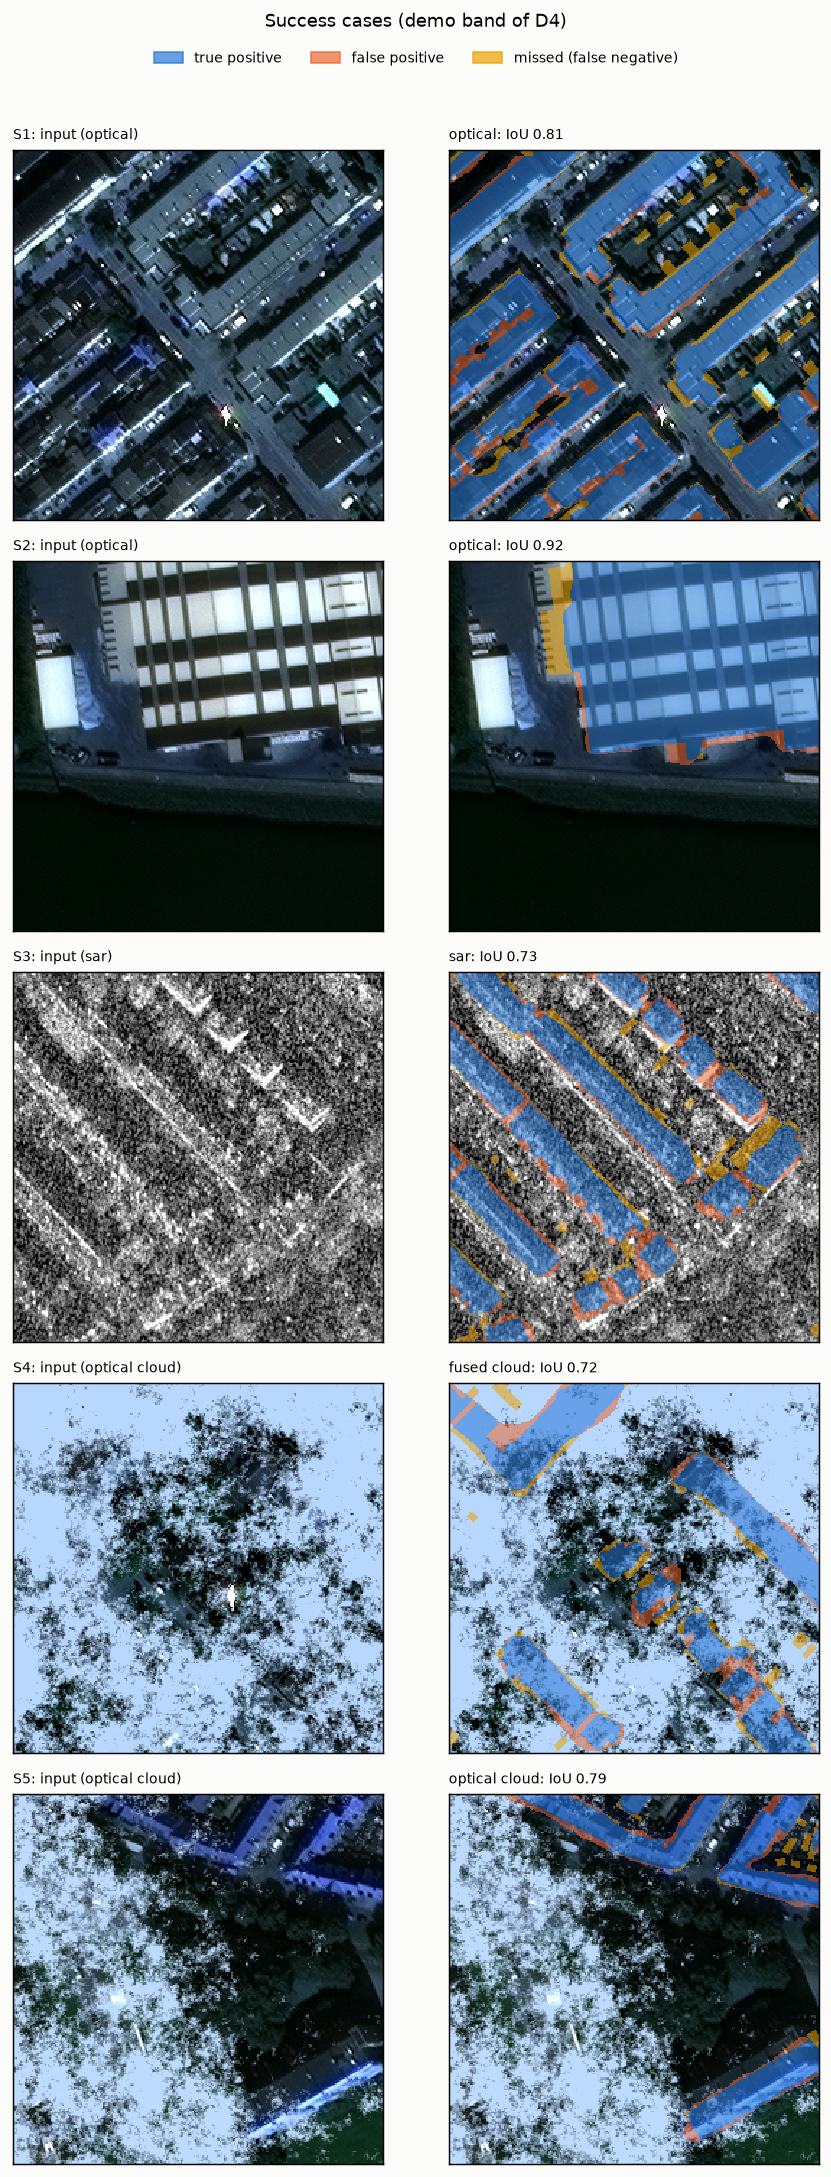
\includegraphics[height=0.92\textheight]{gallery_success.png}
\caption{Success cases S1--S5.}
\label{fig:success}
\end{figure}

\begin{figure}[p]
\centering
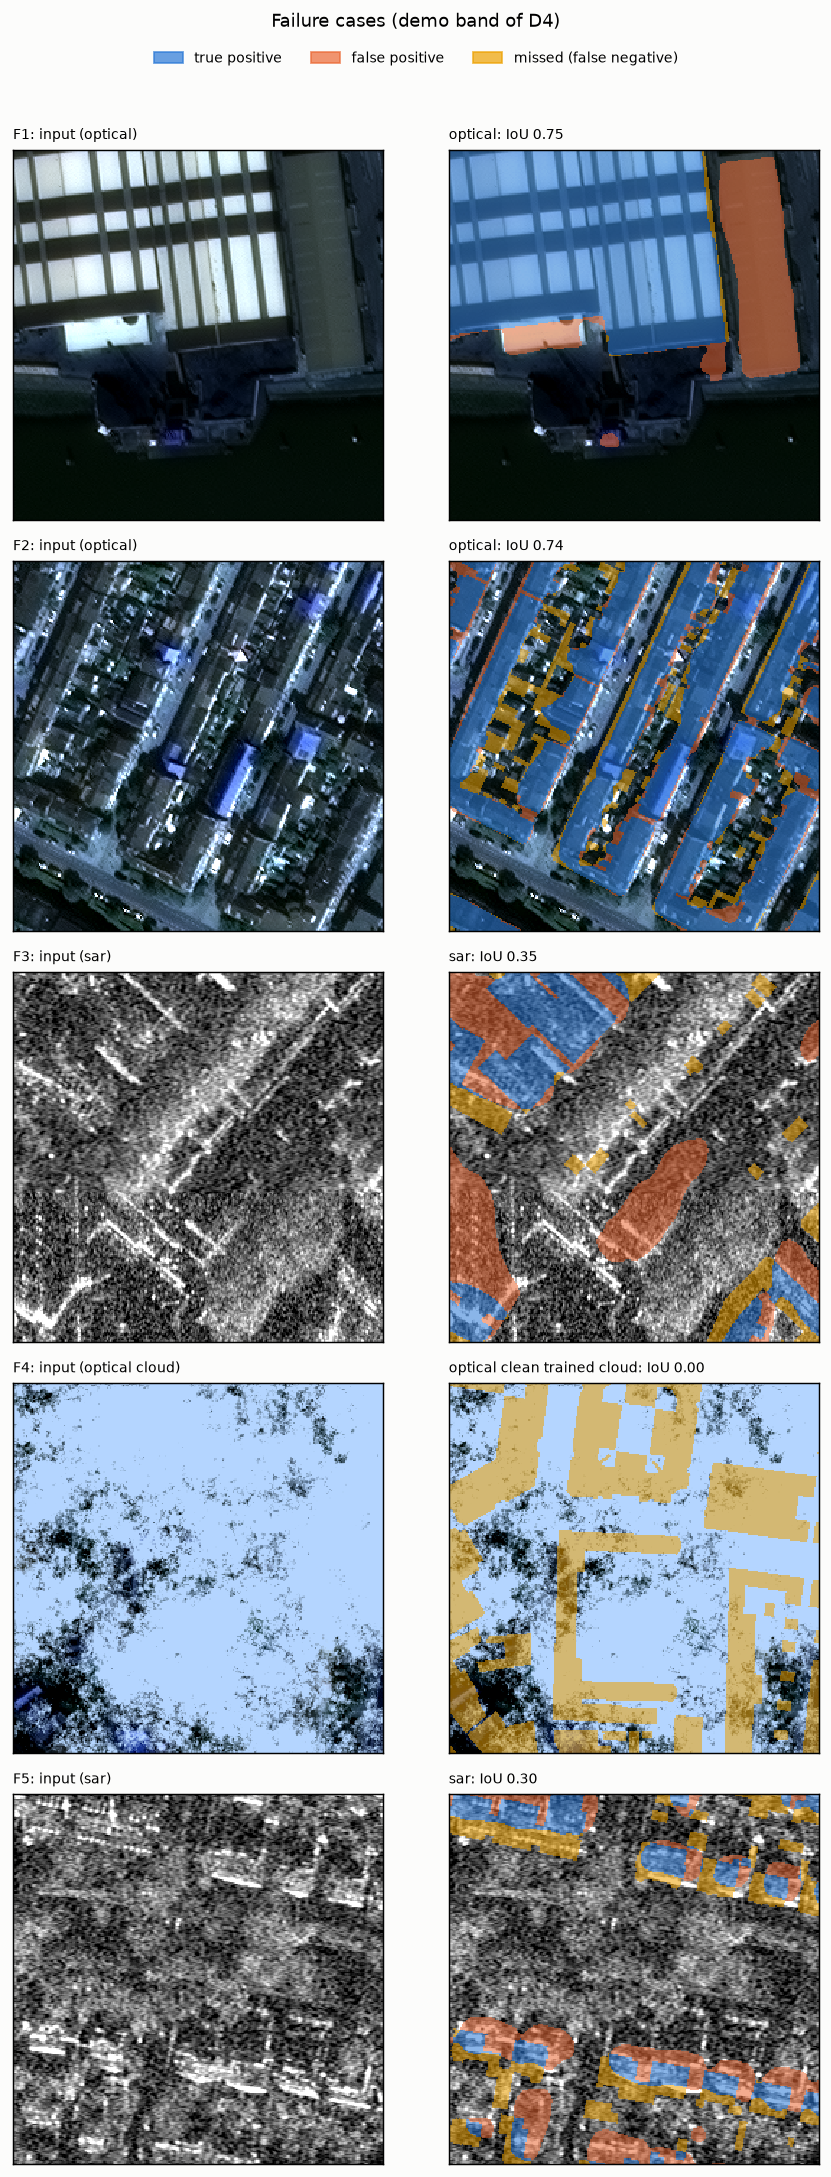
\includegraphics[height=0.92\textheight]{gallery_failure.png}
\caption{Failure cases F1--F5.}
\label{fig:failure}
\end{figure}

\subsection*{Success cases}
\begin{description}
\item[S1 Dense residential block (optical, IoU 0.81).] Twenty-three terraced houses fill
44\,\% of the window. Roof outlines follow the footprints; the errors are a one- to two-pixel
rim along the street edges (orange) and back extensions missed in the shadow of the rows
(yellow). Morphological closing keeps each roof row in one piece, and the 4-connectivity
rule keeps rows that touch at a corner apart.
\item[S2 Large buildings (optical, IoU 0.92).] One industrial hall of 22\,500\,px
(5600\,m$^2$) with a strongly patterned roof is segmented as a single object, so the
skylight stripes are not mistaken for gaps. The only miss is a narrow strip at the hall's
west edge, where the roof is darker.
\item[S3 SAR only (IoU 0.73).] Long rows of houses produce bright double-bounce lines in
the SAR. Because every strip is flipped to the same look direction (D5), the model reads
the bright line and the shadow behind it consistently. Phase correlation finds no offset
between the SAR prediction and the footprints here (0.1, 0.2\,px), so the alignment is
correct.
\item[S4 Fused under cloud (IoU 0.72 vs 0.00).] Clouds cover 71\,\% of the window. The
clean-trained optical model finds nothing (IoU 0.00); the cloud-trained fused model still
recovers 0.72, close to its clear-sky 0.76, because the SAR channels carry the building
structure where the optical channels are white. This is the S3 result at the scale of one
neighbourhood.
\item[S5 Thin cloud, cloud-trained optical (IoU 0.79).] At 34\,\% cover, cloud augmentation
makes the optical model ignore haze and partial cloud: its IoU drops only from 0.81 to
0.79, against 0.70 for the clean-trained model on the same pixels.
\end{description}

\subsection*{Failure cases}
\begin{description}
\item[F1 False positives on a building-like structure (optical).] The window has one
labelled hall. The large orange area is a long, flat, roofed structure next to it (and a
small part of the quay apron) that is not in the label set, giving 7\,500 false-positive
pixels. From above it looks like a roof, but it is not in the labels; the SAR model
barely fires on it (57 false-positive pixels). Whether it is a missing label or a true
error cannot be told from the imagery alone, so this case mixes label ambiguity with model
error. Here the fused model does worse (IoU 0.42), so fusion did not learn to use the SAR
evidence in this case.
\item[F2 Adjacent buildings merged (optical, IoU 0.74).] Nineteen terraced houses with
narrow back yards. In 8 places one predicted component covers three or more labelled
buildings. Gaps of a few pixels between rows are filled by the network and by the
morphological closing, while small rear extensions are missed (yellow). Pixel IoU stays
high, but object F1 drops because one blob matches no single footprint at IoU $\ge 0.5$.
This is the main reason object F1 (0.50) is far below pixel F1 (0.81). Instance-aware
outputs (a boundary class or a distance transform with watershed) are the usual fix.
\item[F3 SAR false detections (IoU 0.35).] The SAR model marks two large blobs over an area
of textured, non-building backscatter (the orange shapes in the lower half) and
mis-places several real buildings. Phase correlation between the prediction and the
footprints finds no consistent shift (peak response 0.06), so this is not a clean layover
offset but bright clutter that looks like building returns. Trees and other rough
surfaces can give high, irregular returns in SAR, which despeckling reduces but does not
remove.
\item[F4 Clean-trained optical under heavy cloud (IoU 0.00).] At 85\,\% cover the
clean-trained model returns nothing for 26 buildings. Under the same clouds the
cloud-trained optical model reaches 0.40 and the fused model 0.47. The failure is the
model never having seen clouds in training, not the sensor alone.
\item[F5 SAR in a dense block (IoU 0.30).] Small houses (465\,px, 116\,m$^2$ on average)
packed in rows. Their double-bounce lines merge and the model outlines the bright lines
rather than the roofs, giving offset outlines and missed rear parts. This window shows the
known limit of SAR building mapping at 0.5\,m (shadow and layover of neighbouring
buildings overlap), and it is why the SAR-only object F1 stays at 0.24--0.26 whatever the
pre-processing.
\end{description}

\paragraph{Stitching seams} are a sixth, solved failure: Fig.~\ref{fig:s1} shows the hard
tile-corner edges of naive stitching that Hann blending removes (S1).


\section{Limitations and future work}
\begin{itemize}
\item \textbf{Split.} The validation split sits next to train, inside the covered extent
(D1). The official SpaceNet~6 Val/Test SAR was not used, so absolute numbers are not
comparable with the challenge leaderboard.
\item \textbf{Look direction.} The service takes one look direction per scene. Mosaics that
mix directions (such as D4) need per-strip handling in the service, as the offline
evaluation already does.
\item \textbf{Clouds.} The clouds are synthetic. Real clouds also cast shadows and change
the haze and colour around them.
\item \textbf{Serving experiments.} These were run on the 4\,GB laptop only, because the
server had no Docker, with 2\,km maximum AOIs and a 4.8\,GB WSL memory limit; the laptop
also warmed up over the session. The resilience (fault injection) experiment and the
Grafana dashboards were left out (Decision D8). With the optical, SAR and fused models
loaded at once, the three ONNX Runtime sessions fill the 4\,GB of GPU memory; capping each
session's memory pool is the next step.
\item \textbf{Future work.} Per-strip SAR statistics computed from the incoming scene
itself; GPU-side normalisation and sigmoid to lift the host bottleneck seen on the server;
a capped GPU memory pool per model; a second task (e.g.\ flood mapping) to exercise
multi-model routing; and a Kubernetes deployment with two workers.
\end{itemize}

\section{Reproducibility}
Code, configurations, request files and figure scripts are in the Git repository; data and
models are versioned with DVC. Milestones are tagged \texttt{v0.1-dip}, \texttt{v0.2-models},
\texttt{v0.3-service}, \texttt{v0.4-bench} and \texttt{v1.0-submission}. Every figure in this
report is written by a committed script (\texttt{make figures}). The README lists the
commands for each phase; \texttt{docs/decisions.md} records every deviation from the plan,
and \texttt{docs/experiments.md} every run.

\begin{thebibliography}{9}\small
\bibitem{shermeyer2020sn6} J.~Shermeyer et al., ``SpaceNet 6: Multi-Sensor All Weather
Mapping Dataset,'' \emph{CVPR Workshops}, 2020. arXiv:2004.06500.
\bibitem{ronneberger2015unet} O.~Ronneberger, P.~Fischer, T.~Brox, ``U-Net: Convolutional
Networks for Biomedical Image Segmentation,'' \emph{MICCAI}, 2015.
\bibitem{he2016resnet} K.~He, X.~Zhang, S.~Ren, J.~Sun, ``Deep Residual Learning for Image
Recognition,'' \emph{CVPR}, 2016.
\bibitem{lee1980} J.-S.~Lee, ``Digital Image Enhancement and Noise Filtering by Use of
Local Statistics,'' \emph{IEEE Trans.\ PAMI}, 2(2), 1980.
\end{thebibliography}

\end{document}
